\documentclass[a4paper]{article}

\usepackage[margin=1in]{geometry} 
\usepackage{amsmath,amsthm,amssymb}
\usepackage{amssymb}
\usepackage{float}
\usepackage{graphicx}
\usepackage{xcolor}
\usepackage[UKenglish]{isodate}
\origdate
\cleanlookdateon
\usepackage[utf8]{inputenc}
\usepackage[hidelinks]{hyperref}
\usepackage{tikz-cd}
\usepackage{enumitem}
\usepackage{mathtools}
\usepackage{float}
\usepackage{mathrsfs}
\renewcommand{\baselinestretch}{1.5} 
\usepackage[varg]{txfonts}
\usepackage{microtype}
\usepackage{steinmetz}
\usepackage{makecell}
\usepackage{multirow}
\begin{document}
\title{Midterms Revision Guide\\[0.1cm]
    \large 30.102 Electromagnetics \& Applications, Term 5 2020}
\author{Wei Min Cher}
\date{16 Mar 2020}

\maketitle

\tableofcontents

\newpage

\section{W1: Waves and Phasorss}
\subsection{Waves}
\begin{itemize}
    \item At high $f$, the phase plays an important role.
    \item Carry energy through vacuum.
    \begin{itemize}[label=$\circ$]
        \item $\checkmark$: EM waves, $\times$: mechanical waves
    \end{itemize}
    \item Types of waves:
    \begin{itemize}[label=$\circ$]
        \item Transverse waves (displacement $\perp$ direction of wave travel) \quad e.g. EM waves
        \item Longitudinal waves (displacement $\parallel$ direction of wave travel) \quad e.g. sound waves
        \item Surface waves (circular motion) \quad e.g. water, ocean waves
    \end{itemize}
\end{itemize}

\subsection{Time-varying Sinusoidal Waves}
\begin{itemize}
    \item General equation: 
    \begin{center}
    \boxed{y(x, t) = Ae^{-\alpha x}\cos{\left(\omega t -\beta x + \phi_{0}\right)}}
    \end{center}
    \item Parameters:
    \begin{enumerate}
    \item Amplitude, $A$: maximum extent of vibration
    \item Wavelength, $\lambda$: distance between 2 points with same displacement
    \item Time period, $T$: amount of time for particle to travel back to same position
    \item Frequency, $f$: number of periods in 1 second $$f = \frac{1}{T} \quad\text{(Hz)}$$
    \item Phase, $\phi$:
    $$\phi = \frac{2\pi t}{T}-\frac{2\pi x}{\lambda}+\phi_{0}\text{, where }\phi_{0}\text{ is the initial/reference phase}$$
    \item Initial/reference phase, $\phi_{0}$:
    $$\phi_{0} = \arccos{\left(\frac{y(0, 0)}{A}\right)}$$
    \begin{itemize}[label=$\circ$]
        \item $\phi_{0}<0$: phase leading
        \item $\phi_{0}>0$: phase lagging
    \end{itemize}
    \item Phase/propagation velocity, $u_{p}$:
    $$u_{p} = f\lambda =  \frac{\omega}{\beta}\quad\text{(m/s)}$$
    \item Angular frequency/velocity, $\omega$:
    $$\omega = 2\pi f = \frac{2\pi}{T}\quad\text{(rad/s)}$$
    \item Wavenumber, $\beta$:
    $$\beta = \frac{2\pi}{\lambda}\quad\text{(rad/m)}$$
    \item Direction of propagation:
     \begin{itemize}[label=$\circ$]
        \item Positive x-direction: $y(x, t) = Ae^{-\alpha x}\cos{\left(\omega t -\beta x + \phi_{0}\right)}$
        \begin{itemize}[label=\tiny$\blacksquare$]
            \item Signs of $\omega t$ and $\beta x$ are opposite
        \end{itemize}
        \item Negative x-direction: $y(x, t) = Ae^{-\alpha x}\cos{\left(\omega t +\beta x + \phi_{0}\right)}$
        \begin{itemize}[label=\tiny$\blacksquare$]
            \item Signs of $\omega t$ and $\beta x$ are the same
        \end{itemize}
    \end{itemize}
    \item Attenuation factor, $e^{-\alpha x}$: factor that amplitude decreases by
    \begin{itemize}[label=$\circ$]
    \item Attenuation constant of medium, $\alpha$
    \item Units: Neper per meter (Np/m)
    
    \medskip
    
    \begin{center}
        \boxed{\text{Solve for }\alpha\text{ using }\frac{Ae^{-\alpha x_1}}{Ae^{-\alpha x_1}} = \frac{y_1}{y_2}.}
    \end{center}
    \end{itemize}
\end{enumerate}
\end{itemize}

\subsection{Complex Numbers}
\begin{itemize}
    \item Rectangular form: $z = x+jy$ \quad (easier to perform addition and subtraction)
    \begin{itemize}[label=$\circ$]
        \item where $x=\operatorname{Re}(z); \quad y = \operatorname{Im}(z)$
    \end{itemize}
    \item Polar form: $z=|z|e^{j\theta}=|z|\phase{\theta}$ \quad (easier to perform multiplication and division)
    \begin{itemize}[label=$\circ$]
        \item $|z|$: magnitude of z; \quad $\theta$: phase angle; \quad $\phase{\theta}$: shorthand for $e^{j\theta}$
    \end{itemize}
    \item \textbf{Euler's identity}: \boxed{e^{j\theta} =\cos\theta+j\sin\theta}
    \begin{align*}
        \text{Similarly, }\cos\theta = \frac{e^{j\theta}+e^{-j\theta}}{2};\quad \sin\theta = \frac{e^{j\theta}-e^{-j\theta}}{2j}.
    \end{align*}
\end{itemize}

\subsection{Phasors}
\begin{itemize}
    \item Any cosinusoidally time-varying function $z(t)$ can be expressed as 
    $$z(t)=\operatorname{Re}\left[\widetilde{Z}e^{j\omega t}\right],\text{ where }\widetilde{Z}\text{ is the phasor of the instantaneous function }z(t).$$
    \item Time domain voltage across resistors, inductors and capacitors
    \begin{itemize}[label=$\circ$]
        \item Resistors: $v_{R}(t) = Ri(t)\quad \Leftrightarrow \quad v_{R}(t) = R\cdot\operatorname{Re}\left[\widetilde{I}e^{j\omega t}\right]$
        \item Inductors: $v_{L}(t) = L\displaystyle\frac{di(t)}{dt}\quad \Leftrightarrow \quad v_{L}(t) = L\cdot\operatorname{Re}\left[j\omega\widetilde{I}e^{j\omega t}\right]$
        \item Capacitors: $v_{C}(t) = \displaystyle\frac{1}{C}\int i(t)\ dt\quad \Leftrightarrow \quad v_{C}(t) = \frac{1}{C}\cdot\operatorname{Re}\left[\displaystyle\frac{\widetilde{I}}{j\omega}e^{j\omega t}\right]$
    \end{itemize}
\end{itemize}

\newpage
\subsection{Phasor Analysis}
\begin{enumerate}
    \item Adopt a cosine reference.
    \begin{itemize}[label=$\circ$]
        \item e.g. $v_{S}(t) = V_{0}\sin\left(\omega t+\phi_{0}\right)= V_{0}\cos\left(\displaystyle\frac{\pi}{2}-\omega t+\phi_{0}\right)= V_{0}\cos\left(\omega t+\phi_{0}-\displaystyle\frac{\pi}{2}\right)$
    \end{itemize}
    \item Express time-dependent variables as phasors.
    \item Write equation in phasor form.
    \item Solve phasor domain equation.
    \item Find instantaneous value.
    \begin{align*}
        i(t) &= \operatorname{Re}\left[\widetilde{I}e^{j\omega t}\right]
    \end{align*}
\end{enumerate}

\subsection{Impedance}
\begin{itemize}
    \item Ratio of phasor voltage across element to phasor current through element, 
    $Z = \displaystyle\frac{\widetilde{V}}{\widetilde{I}}$
    \item Impedance of resistors, inductors and capacitors
    \begin{itemize}[label=$\circ$]
        \item Resistor: $Z_R = R$
        \item Inductor: $Z_L = j\omega L$
        \item Capacitor: $Z_C = \displaystyle\frac{1}{j\omega C}$
    \end{itemize}
\end{itemize}

\newpage
\section{W2: Antennas I}
Definition of antenna: a transducer that converts guided wave on TL $\Leftrightarrow$ EM wave in free space
\subsection{Properties}
\begin{enumerate}
    \item Reciprocity: Same radiation pattern for reception and transmission on 3 conditions:
    \begin{enumerate}
        \item Materials used for the antennas are linear.
        \item Wave propogation medium is linear.
        \item Transmit and receive modes of antenna are polarization matched.
    \end{enumerate}
    \item Transmission Line Equivalent Circuit
    \begin{figure}[H]
        \centering
        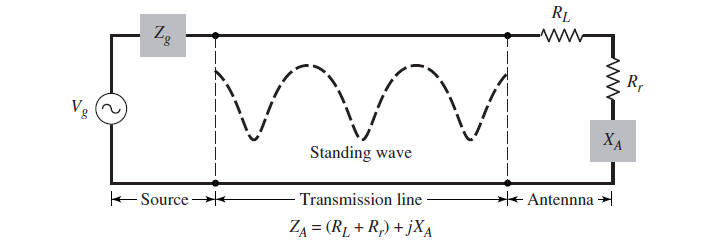
\includegraphics[width=0.7\textwidth]{TL_ant_Tx.png}
        \caption{Transmission-line equivalent circuit of antenna from Balanis' \textit{Antenna Theory} (2016)}
        \label{fig:TLCircTx}
    \end{figure}
    \item Radiation efficiency, $\xi$
    $$\xi = \frac{P_\text{rad}}{P_\text{t}}$$
    \begin{itemize}[label=$\circ$]
        \item where $P_\text{rad}$ is the radiated power,
        \item and $P_\text{t}$ is the transmitter power.
    \end{itemize}
\end{enumerate}

\subsection{Antenna Field Regions}
Letting $D$ be the largest dimension of the antenna and $\lambda$ be the wavelength, they are:
\begin{enumerate}
    \item Reactive near-field region: at a distance $R$, where $0<R<0.62\sqrt{\displaystyle\frac{D^3}{\lambda}}$
    \item Radiating near-field (Fresnel) region: at distance R, where $0.63\sqrt{\displaystyle\frac{D^3}{\lambda}}<R<\displaystyle\frac{2D^2}{\lambda}$
    \item Far-field (Fraunhofer) region: at a distance R, where $R>\displaystyle\frac{2D^2}{\lambda}$
\end{enumerate}

\subsection{Far Field Approximation}
\begin{itemize}
    \item Near radiation source: spherical wavefronts
    \item Far field: approximated as plane waves
\end{itemize}

\subsection{Radiation Mechanism}
\begin{itemize}
    \item To create radiation, there must be:
    \begin{itemize}[label=$\circ$]
        \item either a time-varying current,
        \item or an acceleration/deceleration of charge.
    \end{itemize}
    \item Electric charges needed to excite fields but not sustain them.
\end{itemize}

\subsection{Hertzian Dipole}
\begin{itemize}
    \item A thin, linear conductor with a length $\ell$, where $\ell <  \displaystyle\frac{\lambda}{50}$
    \item Current $i(t)$ is constant along the wire
    \item Current $i(t) = 0$ at the ends of the wire
\end{itemize}

\newpage
\section{W3: Transmission Lines}
\subsection{Unbounded \& Guided Waves}
\begin{itemize}
    \item Unbounded waves
    \begin{itemize}[label=$\circ$]
        \item Propagate in a homogeneous medium
        \item No obstacles
        \item No material interface
    \end{itemize}
    \item Guided waves
    \begin{itemize}[label=$\circ$]
        \item Propagate along a material surface/structure
        \item e.g. coax cable $<$30 GHz, waveguide 5-100 GHz
    \end{itemize}
\end{itemize}

\subsection{Transmission Lines}
\begin{itemize}
    \item Can be classified into 2 types:
    \begin{enumerate}
        \item Transverse electromagnetic (TEM) transmission lines
        \begin{itemize}[label=\tiny$\blacksquare$]
            \item Electric and magnetic fields transverse to direction of propagation
            \item Non-transverse fields negligible
            \item Common feature: 2 $\parallel$ conducting surfaces
            \item e.g. coaxial line, two-wire line, parallel-plate line, strip line, microstrip line, coplanar waveguide, etc.
        \end{itemize}
        \item Higher-order transmission lines
        \begin{itemize}[label=\tiny$\blacksquare$]
            \item $\geq$ 1 significant field component in direction of propagation
            \item e.g. rectangular waveguide, optical fibre, etc.
        \end{itemize}
    \end{enumerate}
\end{itemize}

\newpage
\subsection{Distributed Transmission Line Model}
\begin{center}
\tikzset{every picture/.style={line width=0.75pt}} %set default line width to 0.75pt        

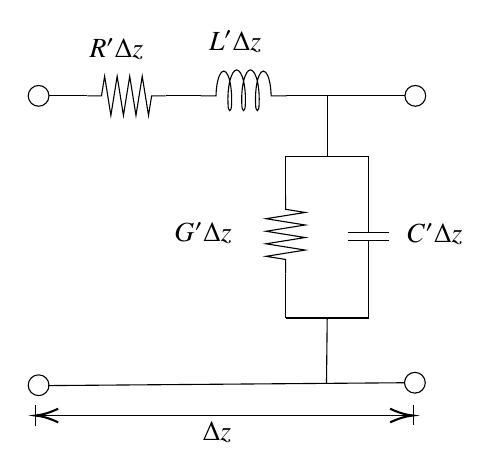
\begin{tikzpicture}[x=0.75pt,y=0.75pt,yscale=-1,xscale=1]
%uncomment if require: \path (0,300); %set diagram left start at 0, and has height of 300

%Shape: Circle [id:dp8563486614412199] 
\draw   (96.5,51.38) .. controls (96.5,48.61) and (98.74,46.38) .. (101.5,46.38) .. controls (104.26,46.38) and (106.5,48.61) .. (106.5,51.38) .. controls (106.5,54.14) and (104.26,56.38) .. (101.5,56.38) .. controls (98.74,56.38) and (96.5,54.14) .. (96.5,51.38) -- cycle ;
%Straight Lines [id:da16692794129708366] 
\draw    (106.5,51.38) -- (125,51.38) ;
%Shape: Resistor [id:dp18098621441023988] 
\draw   (125,51.38) -- (131.79,51.38) -- (133.31,41.94) -- (136.32,60.81) -- (139.35,41.94) -- (142.37,60.81) -- (145.39,41.94) -- (148.41,60.81) -- (151.43,41.94) -- (154.45,60.81) -- (155.95,51.38) -- (162.75,51.38) ;
%Straight Lines [id:da4609625953165635] 
\draw    (162.75,51.38) -- (179.5,51.38) ;
%Straight Lines [id:da8531128972396795] 
\draw    (220.5,51.38) -- (278,51.38) ;
%Shape: Circle [id:dp4781047705271171] 
\draw   (278,51.38) .. controls (278,48.61) and (280.24,46.38) .. (283,46.38) .. controls (285.76,46.38) and (288,48.61) .. (288,51.38) .. controls (288,54.14) and (285.76,56.38) .. (283,56.38) .. controls (280.24,56.38) and (278,54.14) .. (278,51.38) -- cycle ;
%Straight Lines [id:da1299815201883101] 
\draw    (240.5,51.5) -- (240.5,80.25) ;
%Straight Lines [id:da016426728748035302] 
\draw    (220.5,80.5) -- (260.5,80.5) ;
%Straight Lines [id:da2647938683720319] 
\draw    (220.5,80.5) -- (220.5,99.25) ;
%Shape: Inductor (Air Core) [id:dp8447155384806999] 
\draw   (179.5,51.38) -- (186.97,51.38) .. controls (187.08,46.1) and (188.11,41.6) .. (189.58,40.02) .. controls (191.05,38.45) and (192.65,40.12) .. (193.61,44.25) .. controls (194.35,47.46) and (194.65,51.62) .. (194.44,55.65) .. controls (194.44,57.23) and (194.07,58.5) .. (193.61,58.5) .. controls (193.15,58.5) and (192.78,57.23) .. (192.78,55.65) .. controls (192.57,51.62) and (192.87,47.46) .. (193.61,44.25) .. controls (194.47,40.82) and (195.67,38.88) .. (196.93,38.88) .. controls (198.19,38.88) and (199.39,40.82) .. (200.25,44.25) .. controls (200.99,47.46) and (201.29,51.62) .. (201.08,55.65) .. controls (201.08,57.23) and (200.71,58.5) .. (200.25,58.5) .. controls (199.79,58.5) and (199.42,57.23) .. (199.42,55.65) .. controls (199.21,51.62) and (199.51,47.46) .. (200.25,44.25) .. controls (201.11,40.82) and (202.31,38.88) .. (203.57,38.88) .. controls (204.83,38.88) and (206.03,40.82) .. (206.89,44.25) .. controls (207.63,47.46) and (207.93,51.62) .. (207.72,55.65) .. controls (207.72,57.23) and (207.35,58.5) .. (206.89,58.5) .. controls (206.43,58.5) and (206.06,57.23) .. (206.06,55.65) .. controls (205.85,51.62) and (206.15,47.46) .. (206.89,44.25) .. controls (207.85,40.12) and (209.45,38.45) .. (210.92,40.02) .. controls (212.39,41.6) and (213.42,46.1) .. (213.53,51.38) -- (221,51.38) ;
%Straight Lines [id:da5770237917268171] 
\draw    (260.5,80.5) -- (260.5,99.25) ;
%Shape: Resistor [id:dp43249309684418713] 
\draw   (220.5,99.25) -- (220.5,106.04) -- (229.94,107.56) -- (211.06,110.57) -- (229.94,113.6) -- (211.06,116.62) -- (229.94,119.64) -- (211.06,122.66) -- (229.94,125.68) -- (211.06,128.7) -- (220.5,130.2) -- (220.5,137) ;
%Shape: Capacitor [id:dp12918100158392143] 
\draw   (260.5,99.25) -- (260.5,117.16) (270.45,121.14) -- (250.55,121.14) (270.45,117.16) -- (250.55,117.16) (260.5,121.14) -- (260.5,139.05) ;
%Straight Lines [id:da788194267686757] 
\draw    (220.5,137) -- (220.5,158.4) ;
%Straight Lines [id:da6947128647329706] 
\draw    (260.5,139.05) -- (260.5,158.4) ;
%Straight Lines [id:da5905769241393777] 
\draw    (220.5,158.4) -- (260.6,158.4) ;
%Straight Lines [id:da7073937534729144] 
\draw    (240.55,158.4) -- (240.2,190) ;
%Shape: Circle [id:dp8243902142446977] 
\draw   (96.5,190.8) .. controls (96.5,188.04) and (98.74,185.8) .. (101.5,185.8) .. controls (104.26,185.8) and (106.5,188.04) .. (106.5,190.8) .. controls (106.5,193.56) and (104.26,195.8) .. (101.5,195.8) .. controls (98.74,195.8) and (96.5,193.56) .. (96.5,190.8) -- cycle ;
%Straight Lines [id:da11927768041312858] 
\draw    (106.1,190.98) -- (277.8,189.6) ;
%Shape: Circle [id:dp9424629038252774] 
\draw   (277.8,189.6) .. controls (277.8,186.84) and (280.04,184.6) .. (282.8,184.6) .. controls (285.56,184.6) and (287.8,186.84) .. (287.8,189.6) .. controls (287.8,192.36) and (285.56,194.6) .. (282.8,194.6) .. controls (280.04,194.6) and (277.8,192.36) .. (277.8,189.6) -- cycle ;
%Straight Lines [id:da03916929881719011] 
\draw    (100,200.4) -- (100,210.4) ;
%Straight Lines [id:da7595273935248419] 
\draw    (282,200.2) -- (282,210.2) ;
%Straight Lines [id:da09313338412444838] 
\draw    (102,205.4) -- (279.8,205.4) ;
\draw [shift={(281.8,205.4)}, rotate = 180] [color={rgb, 255:red, 0; green, 0; blue, 0 }  ][line width=0.75]    (10.93,-3.29) .. controls (6.95,-1.4) and (3.31,-0.3) .. (0,0) .. controls (3.31,0.3) and (6.95,1.4) .. (10.93,3.29)   ;
\draw [shift={(100,205.4)}, rotate = 0] [color={rgb, 255:red, 0; green, 0; blue, 0 }  ][line width=0.75]    (10.93,-3.29) .. controls (6.95,-1.4) and (3.31,-0.3) .. (0,0) .. controls (3.31,0.3) and (6.95,1.4) .. (10.93,3.29)   ;

% Text Node
\draw (179.2,207.2) node [anchor=north west][inner sep=0.75pt]    {$\Delta z$};
% Text Node
\draw (124.8,22.2) node [anchor=north west][inner sep=0.75pt]    {$R'\Delta z$};
% Text Node
\draw (182,18.8) node [anchor=north west][inner sep=0.75pt]    {$L'\Delta z$};
% Text Node
\draw (166,111.2) node [anchor=north west][inner sep=0.75pt]    {$G'\Delta z$};
% Text Node
\draw (277.6,111.6) node [anchor=north west][inner sep=0.75pt]    {$C'\Delta z$};
\end{tikzpicture}
\end{center}
\begin{itemize}
    \item 4 transmission line parameters:
    \begin{enumerate}
        \item \textit{R'}: Resistance per unit length in $\Omega$/m
        \item \textit{L'}: Inductance per unit length in H/m
        \item \textit{G'}: Conductance per unit length in S/m
        \item \textit{C'}: Capacitance per unit length in F/m
    \end{enumerate}
    \item Geometric parameters
    \begin{itemize}[label=$\circ$]
    \item Coaxial line
    \begin{itemize}[label=\tiny$\blacksquare$]
        \item \textit{a}: Outer radius of inner conductor in m
        \item \textit{b}: Inner radius of outer conductor in m
    \end{itemize}
    \item Two-wire line
    \begin{itemize}[label=\tiny$\blacksquare$]
        \item \textit{d}: Diameter of each line in m
        \item \textit{D}: Spacing between the centers of the wires in m
    \end{itemize}
    \item Parallel-plate line
    \begin{itemize}[label=\tiny$\blacksquare$]
        \item \textit{w}: Width of each plate in m
        \item \textit{h}: Thickness of insulation between plates in m
    \end{itemize}
    \end{itemize}
    \item Constitutive parameters
    \begin{itemize}[label=$\circ$]
    \item Conductors
    \begin{itemize}[label=\tiny$\blacksquare$]
        \item $\mu_c$: Magnetic permeability of conductors
        \item $\sigma_c$: Electrical conductivity of conductors
    \end{itemize}
    \item Insulators
    \begin{itemize}[label=\tiny$\blacksquare$]
        \item $\epsilon$: Electrical permittivity of insulating material
        \item $\mu$: Magnetic permeability of insulating material
        \item $\sigma$: Electrical conductivity of insulating material
    \end{itemize}
    \end{itemize}
\end{itemize}

\subsubsection{Surface Resistance and Other Useful Relations}
\begin{itemize}
    \item Surface Resistance, $R_s = \sqrt{\displaystyle\frac{\pi f\mu_c}{\sigma_c}}$
    \item Perfect conductor: $\sigma_c = \infty$, $\Rightarrow R_s$ and R' = 0.
    \item Perfect dielectric: $\sigma = 0$, $\Rightarrow G' = 0$.
    \item Air line:  $\epsilon = \epsilon_0$, $\mu = \mu_0$, $\sigma = 0$, G' = 0.
    \item All TEM transmission lines have the following relationships:
    \begin{align*}
        L'C' &= \mu\epsilon\\
        \frac{G'}{C'} &= \frac{\sigma}{\epsilon}
    \end{align*}
\end{itemize}

\subsubsection{Summary for Distributed Transmission Line Model}
\begin{table}[H]
\setcellgapes{5pt}
\centering\makegapedcells
\begin{tabular}{|c|c|c|c|c|}
\hline
\textbf{Parameter} & \textbf{Coaxial} & \textbf{Two-Wire} & \textbf{Parallel-Plate} & \textbf{Unit} \\ \hline
R' & $\displaystyle\frac{R_s}{2\pi}\left(\frac{1}{a}+\frac{1}{b}\right)$ & $\displaystyle\frac{2R_s}{\pi d}$ & $\displaystyle\frac{2R_s}{w}$     & $\Omega$/m    \\ \hline
L' & $\displaystyle\frac{\mu}{2\pi}\text{ln}\frac{b}{a}$ & $\displaystyle\frac{\mu}{\pi}\text{ln}\left[\frac{D}{d}+\sqrt{\left(\frac{D}{d}\right)^2-1}\ \right]$ & $\displaystyle\frac{\mu h}{w}$ & H/m           \\ \hline
G' & $\displaystyle\frac{2\pi\sigma}{\text{ln}\left(\displaystyle\frac{b}{a}\right)}$ & $\displaystyle\frac{\pi\sigma}{\text{ln}\left[\displaystyle\frac{D}{d}+\sqrt{\left(\displaystyle\frac{D}{d}\right)^2-1}\ \right]}$ & $\displaystyle\frac{\sigma w}{h}$ & S/m           \\ \hline
C' &   $\displaystyle\frac{2\pi\epsilon}{\text{ln}\left(\displaystyle\frac{b}{a}\right)}$ &  $\displaystyle\frac{\pi\epsilon}{\text{ln}\left[\displaystyle\frac{D}{d}+\sqrt{\left(\displaystyle\frac{D}{d}\right)^2-1}\ \right]}$ &  $\displaystyle\frac{\epsilon w}{h}$ & F/m           \\ \hline
\end{tabular}
\end{table}

\subsection{Transmission Line Equations}
\begin{center}
    \boxed{
        \begin{array}{ccc}
            -\displaystyle\frac{\partial v(z, t)}{\partial z} = R'\ i(z, t)+L'\ \displaystyle\frac{\partial i(z, t)}{\partial t} & \Leftrightarrow & -\displaystyle\frac{\partial \widetilde{V}(z)}{\partial z} = (R'+j\omega L')\widetilde{I}(z)\\[8pt]
            \medskip
            -\displaystyle\frac{\partial i(z, t)}{\partial z} = G'\ v(z, t)+C'\ \displaystyle\frac{\partial v(z, t)}{\partial t} & \Leftrightarrow & -\displaystyle\frac{\partial \widetilde{I}(z)}{\partial z} = (G'+j\omega C')\widetilde{V}(z)
        \end{array}
    }
\end{center}

\subsection{Characteristic Parameters}
\subsubsection{Propagation Constant}
$$\gamma = \sqrt{(R'+j\omega L')(G'+j\omega C')} = \alpha + j\beta$$
\begin{itemize}
    \item $\gamma$: complex propagation constant
    \item $\alpha$: attenuation constant in Np/m
    \item $\beta$: phase constant in rad/m
\end{itemize}

\subsubsection{Characteristic Impedance}
\begin{center}
    $Z_0 = \displaystyle\frac{V_0^+}{I_0^+} = \displaystyle\frac{-V_0^-}{I_0^-} = \sqrt{\displaystyle\frac{R'+j\omega L'}{G'+j\omega C'}}$ in units of $\Omega$
\end{center}

\subsubsection{Summary for Characteristic Parameters}
\begin{table}[H]
\setcellgapes{5pt}
\centering\makegapedcells
\begin{tabular}{|l|c|c|c|}
\hline
 & \textbf{\begin{tabular}[c]{@{}c@{}}Propagation constant\\ $\gamma = \alpha + j\beta$\end{tabular}} & \textbf{\begin{tabular}[c]{@{}c@{}}Phase velocity\\ $u_p$\end{tabular}} & \textbf{\begin{tabular}[c]{@{}c@{}}Characteristic impedance\\ $Z_0$\end{tabular}} \\ \hline
\textbf{General case} & $\sqrt{(R'+j\omega L')(G'+j\omega C')}$ & $\displaystyle{\frac{\omega}{\beta}}$ & $\sqrt{\displaystyle\frac{R'+j\omega L'}{G'+j\omega C'}}$ \\ \hline
\textbf{Lossless (R' = G' = 0)} & \multirow{7}{*}{$\alpha = 0,\ \beta = \displaystyle\frac{\omega\sqrt{\epsilon_r}}{c}$} & \multirow{7}{*}{$\displaystyle\frac{c}{\sqrt{\epsilon_r}}$} & $\sqrt{\displaystyle\frac{L'}{C'}}$ \\ \cline{1-1} \cline{4-4} 
\textbf{Lossless coaxial} &  &  & $\displaystyle\frac{60}{\sqrt{\epsilon_r}}\ln \frac{b}{a}$ \\ \cline{1-1} \cline{4-4} 
\textbf{Lossless two wire} &  &  & \begin{tabular}[c]{@{}c@{}}$\displaystyle\frac{120}{\sqrt{\epsilon_r}}\ln \left[\frac{D}{d}+\sqrt{\frac{D}{d}^2-1}\right]$\\ If D $\gg$ d, $\approx\displaystyle\frac{120}{\sqrt{\epsilon_r}}\ln\displaystyle\frac{2D}{d}$\end{tabular} \\ \cline{1-1} \cline{4-4} 
\textbf{Lossless $\parallel$ plate} &  &  & $\displaystyle\frac{120\pi}{\sqrt{\epsilon_r}}\frac{h}{w}$ \\ \hline
\end{tabular}
\end{table}

\subsection{Dispersion \& Guided Wavelength}
\begin{itemize}
    \item Dispersion: phase velocity of wave depends on its frequency
    \begin{itemize}[label=$\circ$]
        \item $\checkmark$: Dispersive media, $\times$: non-dispersive media
        \item Degree of distortion $\propto$ length of dispersive line
    \end{itemize}
    \item Guided wavelength, $\lambda_g$: distance between two equal phase planes along the transmission line
    $$\lambda_g = \frac{c}{f\sqrt{\epsilon_r}} = \frac{\lambda_0}{\sqrt{\epsilon_r}}$$
\end{itemize}

\newpage
\subsection{Standing Waves \& Standing Wave Pattern}
\begin{itemize}
    \item Standing wave: formed when two waves on transmission line propagating in opposite directions
    \item Standing wave patterns: sinusoidal patterns caused by interference of two travelling waves
    \begin{align*}
        \widetilde{V}(z) &= \widetilde{V}^+(z)+\widetilde{V}^-(z) = V_0^+e^{-\gamma z} + V_0^-e^{\gamma z}\\
        \widetilde{I}(z) &= \widetilde{I}^+(z)+\widetilde{I}^-(z) = I_0^+e^{-\gamma z} + I_0^-e^{\gamma z}
    \end{align*}
    \begin{itemize}[label=$\circ$]
        \item Using either one of the two axes:
        \begin{itemize}[label=\tiny$\blacksquare$]
            \item $z$-axis: load at $z=0$, generator at $z=-l$
            \item $d$-axis: load at $d=0$, generator at $d=l$
        \end{itemize}
        \item Affected by:
        \begin{itemize}[label=\tiny$\blacksquare$]
            \item Relation of $\widetilde{V}^-(z)$ and $\widetilde{V}^+(z)$ at $z=0$
            \item Relation of $V_0^+$ and $V_0^-$
        \end{itemize}
    \end{itemize}
    \item Magnitude of voltage, $|\widetilde{V}(d)|= |V_0^+|\left[1+|\Gamma|^2+2|\Gamma|\cos(2\beta d-\theta_r)\right]^{1/2}$
    \item Magnitude of current, $|\widetilde{I}(d)| = \displaystyle\frac{|V_0^+|}{Z_0}\left[1+|\Gamma|^2+2|\Gamma|\cos(2\beta d-\theta_r)\right]^{1/2}$
    \item Voltage maximum, $d_{max}$: distance from load where $|\widetilde{V}(d)|$ is a maximum
    \begin{align*}
        d_{max} &= \frac{\theta_r}{4\pi}+\frac{n\lambda}{2},\ \begin{cases}
        \quad n = 1, 2, \ldots & \text{if }\theta_r < 0\\
        \quad n = 0, 1, 2, \ldots & \text{if }\theta_r \geq 0
        \end{cases}
    \end{align*}
    \item Voltage minimum, $d_{min}$: distance from load where $|\widetilde{V}(d)|$ is a minimum
    \begin{align*}
        d_{min} = \begin{cases}
        \quad d_{max} + \displaystyle\frac{\lambda}{4}, & \text{if }d_{max} < \displaystyle\frac{\lambda}{4}\\[0.2cm]
        \quad d_{max} - \displaystyle\frac{\lambda}{4}, & \text{if }d_{max} \geq \displaystyle\frac{\lambda}{4}
        \end{cases}
    \end{align*}
    \item Voltage standing wave ratio (VSWR), $S = \displaystyle\frac{|\widetilde{V}|_{max}}{|\widetilde{V}|_{min}} = \displaystyle\frac{1+|\Gamma|}{1-|\Gamma|}$ (dimensionless)
\end{itemize}

\newpage
\subsection{Reflection Coefficient}
\begin{itemize}
    \item Ratio of reflected and incident voltages at the load. \quad $\displaystyle\frac{I_0^-}{I_0^+} = -\displaystyle\frac{V_0^-}{V_0^+} = -\Gamma_L$
    \item A complex quantity. \quad $\Gamma_L =  |\Gamma_L|e^{j\theta_r} = \displaystyle\frac{V_0^-}{V_0^+} = \displaystyle\frac{Z_L-Z_0}{Z_L+Z_0}= \displaystyle\frac{z_L-1}{z_L+1}$ (dimensionless)
    \item Normalized load impedance, $z_L = \displaystyle\frac{Z_L}{Z_0}$ (dimensionless)
\end{itemize}
\begin{table}[H]
\setcellgapes{5pt}
\centering\makegapedcells
\begin{tabular}{c|c|c}
\textbf{Load} & \textbf{$|\Gamma|$} & \textbf{$\theta_r$} \\ \hline
$Z_L = (r+jx)Z_0$ & $\sqrt{\displaystyle\frac{(r-1)^2+x^2}{(r+1)^2+x^2}}$ & $\tan^{-1}\left(\displaystyle\frac{x}{r-1}\right)-\tan^{-1}\left(\displaystyle\frac{x}{r+1}\right)$ \\
$Z_L = Z_0$ & 0 & NA \\
$Z_L =$ short-circuit & 1 & $\pm 180^\circ$ \\
$Z_L =$ open-circuit & 1 & 0 \\
$Z_L = jX = j\omega L$ (capacitor) & 1 & $\pm 180^\circ - 2\tan^{-1}(X)$ \\
$Z_L = jX = -\displaystyle\frac{j}{\omega C}$ & 1 & $\pm 180^\circ + 2\tan^{-1}(X)$                     
\end{tabular}
\end{table}

\subsection{Wave Impedance}
$$Z(d) = \frac{\widetilde{V}(d)}{\widetilde{I}(d)} = Z_0\left(\frac{1+\Gamma_d}{1-\Gamma_d}\right)$$
\begin{itemize}
    \item Phase-shifted voltage reflection coefficient $\Gamma_d = |\Gamma|e^{j(\theta_r-2\beta d)}$
\end{itemize}

\subsection{Input Impedance}
\begin{align*}
    Z_{\text{in}} &= Z_0\left(\frac{z_L\cos\beta l+j\sin \beta l}{\cos\beta l+jz_L\sin\beta l}\right)\\
    &= Z_0\left(\frac{z_L+j\tan\beta l}{1+jz_L\tan\beta l}\right)\\
    V_0^+ &= \left(\frac{\widetilde{V}_{g}Z_\text{in}}{Z_g+Z_\text{in}}\right)\left(\frac{1}{e^{j\beta l}+\Gamma e^{-j\beta l}}\right)
\end{align*}

\newpage
\subsection{Short-Circuited Line}
\begin{itemize}
    \item $\Gamma$ = -1,\ $S = \infty$
    \item $\widetilde{V}_\text{sc}(d) =  V_0^+\left(e^{j\beta d}-e^{-j\beta d}\right) = 2jV_0^+\sin\beta d$
    \item $\widetilde{I}_\text{sc}(d) = \displaystyle\frac{V_0^+}{Z_0}\left(e^{j\beta d}+e^{-j\beta d}\right) = \displaystyle\frac{2V_0^+}{Z_0}\cos\beta d$
    \item $Z_\text{sc}(d) = \displaystyle\frac{\widetilde{V}_\text{sc}(d)}{\widetilde{I}_\text{sc}(d)} = jZ_0\tan\beta d$
    \item By choosing $\ell$, can make $L$ and $C$ of any reactance.
    \begin{itemize}[label=$\circ$]
        \item If $\tan\beta l \geq 0$, $jZ_0\tan\beta l = j\omega L_\text{eq}$.
        \item If $\tan\beta l \leq 0$, $jZ_0\tan\beta l = \displaystyle\frac{1}{j\omega C_\text{eq}}$.
    \end{itemize}
\end{itemize}

\subsection{Open-Circuited Line}
\begin{itemize}
    \item $\Gamma$ = 1,\ $S = \infty$
    \item $\widetilde{V}_\text{oc}(d) = V_0^+\left(e^{j\beta d}+e^{-j\beta d}\right) = 2V_0^+\cos\beta d$
    \item $\widetilde{I}_\text{oc}(d) = \displaystyle\frac{V_0^+}{Z_0}\left(e^{j\beta d}-e^{-j\beta d}\right) = \displaystyle\frac{2jV_0^+}{Z_0}\sin\beta d$
    \item $Z_\text{oc}(d) = \displaystyle\frac{\widetilde{V}_\text{oc}(d)}{\widetilde{I}_\text{oc}(d)} = -jZ_0\cot\beta d$
    \item By choosing $\ell$, can make $L$ and $C$ of any reactance.
    \begin{itemize}[label=$\circ$]
        \item If $Z^\text{oc}_{in} \geq 0$, $-jZ_0\cot\beta l = j\omega L_\text{eq}$.
        \item If $Z^\text{oc}_{in} \geq 0$, $-jZ_0\cot\beta l = \displaystyle\frac{1}{j\omega C_\text{eq}}$.
    \end{itemize}
\end{itemize}

\subsection{Measuring Characteristic Impedance and Phase Constant}
$$Z_0 = \sqrt{Z^\text{sc}_\text{in}Z^\text{oc}_\text{in}}$$
$$\tan\beta l = \sqrt{\frac{-Z^\text{sc}_\text{in}}{Z^\text{oc}_\text{in}}}\quad \text{can be used to find }\beta$$

\subsection{Quarter and Half Wavelength TLs}
\begin{itemize}
    \item For a half wavelength TL, where $l = \displaystyle\frac{n\lambda}{2}$, \boxed{Z_\text{in} = Z_\text{L}.}
    \item For a quarter wavelength TL, where $l = \displaystyle\frac{\lambda}{4}+\frac{n\lambda}{2}$, \boxed{Z_\text{in} = \displaystyle\frac{Z_0^2}{Z_\text{L}}.}
\end{itemize}

\newpage
\subsection{Instantaneous Power of a Lossless TL}
\begin{itemize}
    \item $v(d, t) = |V_0^+|\left[\cos(\omega t+\beta d+\phi^+)+|\Gamma|\cos(\omega t-\beta d+\phi^++\theta_r)\right]$
    \item $i(d, t) = \displaystyle\frac{|V_0^+|}{Z_0}\left[\cos(\omega t+\beta d+\phi^+)-|\Gamma|\cos(\omega t-\beta d+\phi^++\theta_r)\right]$
    \item $P(d, t) = \displaystyle\frac{|V_0^+|^2}{Z_0}\left[\cos^2(\omega t+\beta d+\phi^+)-|\Gamma|^2\cos^2(\omega t-\beta d+\phi^++\theta_r)\right]$
    \begin{itemize}[label=$\circ$]
        \item The instantaneous power oscillates at twice the rate of the voltage or current.
    \end{itemize}
    \item Incident power $P^i(d, t) = \displaystyle\frac{|V_0^+|^2}{2Z_0}\left[1+\cos(2\omega t+2\beta d+2\phi^+)\right]$
    \item Reflected power $P^r(d, t) = -|\Gamma|^2\displaystyle\frac{|V_0^+|^2}{2Z_0}\left[1+\cos(2\omega t-2\beta d+2\phi^++2\theta_r)\right]$
\end{itemize}

\subsection{Time-Average Power of a Lossless TL}
\begin{itemize}
    \item Time-average incident power, $P^\text{i}_\text{av} = \displaystyle\frac{|V_0^+|^2}{2Z_0}$ is measured in W.
    \item Time-average reflected power, $P^\text{r}_\text{av} = -|\Gamma|^2\displaystyle\frac{|V_0^+|^2}{2Z_0} = -|\Gamma|^2P^\text{i}_\text{av}$ is measured in W.
    \begin{itemize}
        \item Average reflected power is average incident power diminished by $|\Gamma|^2$.
    \end{itemize}
\end{itemize}

\newpage
\section{W5: Matching Networks}
\subsection{Concept of Matching Networks}
\begin{itemize}
    \item Eliminate reflections for waves incident from source
    \item All power goes to load
    \item May consist of lumped elements i.e. capacitors and inductors, or sections of TLs
\end{itemize}

\subsection{Matching Networks in Series}
\begin{enumerate}
    \item In-series $\lambda$/4 transformer inserted in front of $Z_L$ \quad (if $Z_L$ is real)
    \item In-series $\lambda$/4 transformer inserted at $d = d_\text{max}$ or $d = d_\text{min}$ \quad (if $Z_L$ is complex)
\end{enumerate}

\subsection{Matching Networks in Parallel}
\begin{enumerate}
    \item In-parallel insertion of capacitor at distance $d_1$
    \item In-parallel insertion of inductor at distance $d_2$
    \item In-parallel insertion of a short-circuited stub
\end{enumerate}

\subsection{Lumped Element Matching}
\begin{itemize}
    \item To achieve matched condition, $y_\text{in} = y_\text{d}+y_\text{s}+g_\text{d}+j(b_\text{d}+b_\text{s})= 1+j0$. As such,
    \begin{center}
        \boxed{
        \begin{array}{cc}
            g_\text{d} = 1 & \text{(real condition)}\\
            b_\text{d} = -b_\text{s} & \text{(imaginary condition)}
        \end{array}
    }
    \end{center}
\end{itemize}

\newpage
\section{W5: Smith Chart}
\begin{enumerate}
    \item Complex unit circle
    \item Concentric $r_\text{L}$ circles
    \item $x_\text{L}$ curves
    \item Wavelengths toward generator (WTG) scale \quad (clockwise)
    \item Wavelengths toward load (WTL) scale \quad (counterclockwise)
\end{enumerate}

\subsection{How to Use the Smith Chart}
\begin{itemize}
    \item Read off $\Gamma_\text{L}$ from $z_\text{L}$: $\Gamma_\text{L} = |\Gamma_\text{L}|e^{j\theta_r}$
    \item Constant $\Gamma_L$/SWR circle, move towards WTG/WTL directions
    \item Read off to find distance $d$
    \item Find $Y$ from $Z$
    \begin{itemize}[label=$\circ$]
        \item $y$ opposite from $z$ in SWR circle
        \item $\Rightarrow Y_\text{L} = y_\text{L}\cdot Y_0$ in units of S
    \end{itemize}
\end{itemize}

\newpage
\section{W6: Vector Algebra}
\subsection{Basic Vector Operations}
\begin{itemize}
    \item Unit vector $\hat{a} = \displaystyle\frac{\overrightarrow{A}}{|\overrightarrow{A}|} = \displaystyle\frac{\hat{x}A_x+\hat{y}A_y+\hat{z}A_z}{\sqrt{A_x^2+A_y^2+A_z^2}}$
    \item Position vector: $\overrightarrow{R_1} = \overrightarrow{OP_1}$
    \item Distance vector: $\overrightarrow{R_{12}} = \overrightarrow{P_1P_2} = \overrightarrow{R_2}-\overrightarrow{R_1}$
    \begin{itemize}[label=$\circ$]
        \item Distance $d = |\overrightarrow{R_{12}}|$
    \end{itemize}
    \item Vector addition
    \begin{itemize}[label=$\circ$]
        \item Done graphically using parallelogram or head-to-tail method.
        \item Commutative: $\overrightarrow{A} + \overrightarrow{B} = \overrightarrow{B} + \overrightarrow{A}$
    \end{itemize}
\end{itemize}

\subsection{Dot Product}
$$\overrightarrow{A}\cdot\overrightarrow{B} = AB\cos\theta_\text{AB},\quad \theta_\text{AB} = \cos^{-1}\left(\frac{\overrightarrow{A}\cdot\overrightarrow{B}}{\sqrt{\overrightarrow{A}\cdot\overrightarrow{A}}\cdot\sqrt{\overrightarrow{B}\cdot\overrightarrow{B}}}\right)$$
\begin{itemize}
    \item Commutative and distributive.
        \begin{align*}
            \overrightarrow{A}\cdot\overrightarrow{B} &= \overrightarrow{B}\cdot\overrightarrow{A}\text{ (commutative)}\\
            \overrightarrow{A}\cdot(\overrightarrow{B}+\overrightarrow{C}) &= \overrightarrow{A}\cdot\overrightarrow{B}+\overrightarrow{A}\cdot\overrightarrow{C}\text{ (distributive)}
        \end{align*}
    \item Can be used to find magnitude of vector.
    $$A = |\overrightarrow{A}| = \sqrt{\overrightarrow{A}\cdot\overrightarrow{A}}$$
\end{itemize}

\subsection{Cross Product}
$$\overrightarrow{A}\times\overrightarrow{B} = \hat{n}\ AB\sin\theta_\text{AB},\ \hat{n}\text{ in direction of right hand rule}$$
\begin{itemize}
    \item Anti-commutative and distributive.
    \begin{align*}
        \overrightarrow{A}\times\overrightarrow{B} &= -\overrightarrow{B}\times\overrightarrow{A}\text{ (anti-commutative)}\\
        \overrightarrow{A}\times(\overrightarrow{B}+\overrightarrow{C}) &= \overrightarrow{A}\times\overrightarrow{B}+\overrightarrow{A}\times\overrightarrow{C}\text{ (distributive)}
    \end{align*}
    \item Can be re-expressed as a determinant.
    $$\overrightarrow{A}\times\overrightarrow{B} = \left|
    \begin{array}{ccc}
        \hat{x} & \hat{y} & \hat{z}\\
         A_x & A_y & A_z\\
         B_x & B_y & B_z
    \end{array}\right|$$
\end{itemize}

\subsection{Scalar Triple Product}
$$\overrightarrow{A}\cdot(\overrightarrow{B}\times\overrightarrow{C}) = \overrightarrow{B}\cdot(\overrightarrow{C}\times\overrightarrow{A}) = \overrightarrow{C}\cdot(\overrightarrow{A}\times\overrightarrow{B}) = \left|
    \begin{array}{ccc}
         A_x & A_y & A_z\\
         B_x & B_y & B_z\\
         C_x & C_y & C_z
    \end{array}\right|$$

\subsection{Vector Triple Product}
$$\overrightarrow{A}\times(\overrightarrow{B}\times\overrightarrow{C})$$
\begin{itemize}
    \item Not associative.
    $$\overrightarrow{A}\times(\overrightarrow{B}\times\overrightarrow{C})\neq(\overrightarrow{A}\times\overrightarrow{B})\times\overrightarrow{C}$$
    \item Follows the "bac-cab" rule.
    $$\overrightarrow{A}\times(\overrightarrow{B}\times\overrightarrow{C}) = \overrightarrow{B}(\overrightarrow{A}\cdot\overrightarrow{C})-\overrightarrow{C}(\overrightarrow{A}\cdot\overrightarrow{B})$$
\end{itemize}

\newpage
\appendix
\section{Appendix}
\subsection{Derivatives}
\begin{center}
    $\displaystyle\frac{d}{dt}$\\[0.5cm]
    $\sin\rightarrow\cos,\quad \cos\rightarrow -\sin,\quad \tan\rightarrow\sec^2,\quad x^n\rightarrow nx^{n-1},\quad e^{ax}\rightarrow ae^{ax}, \quad \ln x \rightarrow \displaystyle\frac{1}{x}$
\end{center}
\subsection{Integrals}
\begin{center}
    $\int$\\[0.5cm]
    $\sin\rightarrow -\cos,\quad \cos\rightarrow\sin,\quad \sec^2\rightarrow\tan,\quad x^n\rightarrow\displaystyle\frac{1}{n}x^{n+1},\quad e^{ax}\rightarrow\displaystyle\frac{1}{a}e^{ax},\quad \displaystyle\frac{1}{x}\rightarrow\ln |x|$
\end{center}
\subsection{Integration by Parts}
$$\int u\ dv = uv -\int v du$$
Priority of choosing $u$:
\begin{enumerate}
    \item Logarithmic terms
    \item Inverse trigonometric terms
    \item Algebraic terms
    \item Trigonometric terms
    \item Exponential terms
\end{enumerate}
\subsection{Phasors}
\begin{itemize}
    \item Identities: $\sin x = \cos\left(\displaystyle\frac{\pi}{2}-x\right);\quad\cos(-x) = \cos x$
    \item Voltage across capacitor, $v_C(t)$:
    \begin{align*}
        \int i(t) &= \operatorname{Re}\left[\frac{\widetilde{I}e^{j\omega t}}{j\omega}\right] =  \operatorname{Re}\left[\frac{-j\widetilde{I}e^{j\omega t}}{\omega}\right]=\operatorname{Re}\left[\frac{-\widetilde{I}j\cos\omega t+\widetilde{I}\sin\omega t}{\omega}\right]\\
        &= \frac{\widetilde{I}\sin\omega t}{\omega}\\
        \Rightarrow v_C(t) &= \frac{\int i(t)}{C} = \frac{\widetilde{I}\sin\omega t}{\omega C}
    \end{align*}
    \item Voltage across inductor, $v_L(t)$:
    \begin{align*}
        \frac{di(t)}{dt} &= \operatorname{Re}\left[j\omega \widetilde{I}e^{j\omega t}\right] = \operatorname{Re}\left[j\omega\widetilde{I}\cos\omega t-\widetilde{I}\omega\sin\omega t\right] = -\widetilde{I}\omega \sin\omega t\\
        \Rightarrow v_L(t) &= L\frac{di(t)}{dt} = -L\omega\widetilde{I}\sin\omega t
    \end{align*}
\end{itemize}
\end{document}